\documentclass[10pt]{standalone}
\usepackage{amsmath}
\usepackage{amssymb}
\usepackage{pgf,tikz}
\usepackage{mathrsfs}
\usetikzlibrary{arrows,calc,positioning,shapes.symbols,shapes.geometric,shapes.misc}
\pagestyle{empty}
\usepackage{siunitx}


\begin{document}

	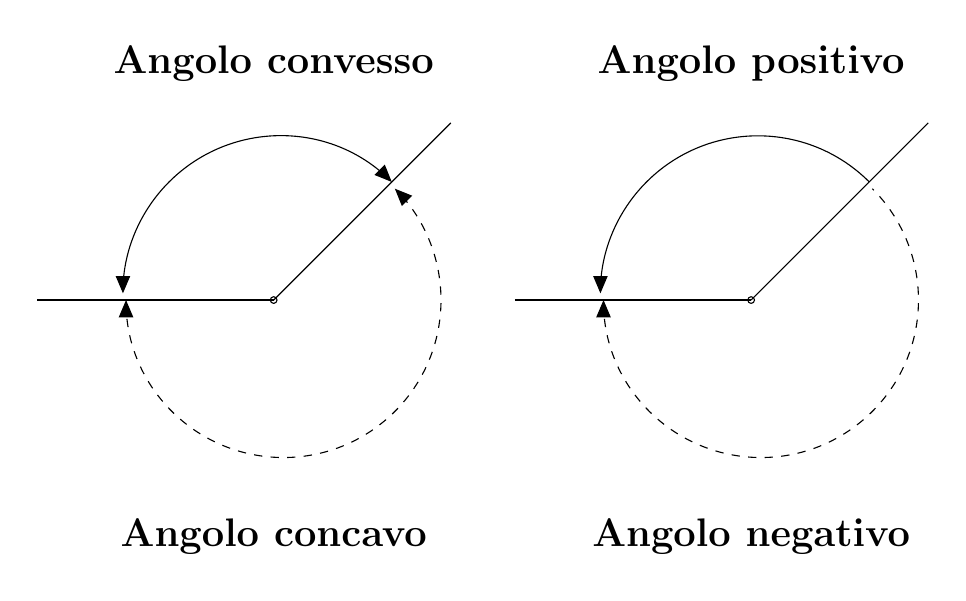
\begin{tikzpicture}[>=triangle  45,x=1.5cm,y=1.5cm]
	\coordinate (C) at (0,0);
	\coordinate (A) at (1.5,1.5);
	\coordinate (B) at (-2,0);
	\matrix[column sep=0.8cm,row sep=0.5cm]{
		\draw (A) - -(C);
		\draw (B) - -(C);
		\draw [<->] (1,1) arc(45:180:2cm);
		\draw [<->, dashed,] (-1.25,0)  arc(-180:45:2cm);
		\node (A1) at (0,2) {\textbf{{\Large Angolo convesso}}};
		\node (A2) at (0,-2) {\textbf{{\Large Angolo concavo}}};
		\node[draw, circle, inner sep=.3mm] (a) at (C) {};&
		\draw (A) - -(C);
		\draw (B) - -(C);
		\draw [->] (1,1) arc(45:180:2cm);
		\draw [<-, dashed,] (-1.25,0)  arc(-180:45:2cm);
		\node (A1) at (0,2) {\textbf{{\Large Angolo positivo}}};
		\node (A2) at (0,-2) {\textbf{{\Large Angolo negativo}}}; 
		\node[draw, circle, inner sep=.3mm] (a) at (C) {};\\
	};
	\end{tikzpicture}
\end{document}